\chapter{GitHub Action UID/GID Resolution}\label{chap:gh_action_build_args}

The containers build with the \cxtoolkit are designed to allow invocation
so that code under scan is isolated from mutation by any malware that
is included in the build scripts or third-party dependencies.  This is
primarily done by mapping volumes to the running container with permissions
on the original source location set to disallow writes.  The permissions
on the source location propagate to the container with a UID/GID that, if not
matched correctly in the container, may not allow the source to be read for
scanning.

GitHub actions execute on either self-hosted runners or GitHub-hosted runners.
Knowing the correct UID/GID to supply in the build args \texttt{GROUP\_ID}
and \texttt{USER\_ID} (documented in Appendix \ref{chap:build_args}) will
allow invocation of \cxtoolkit containers to work correctly on the type of
runner appropriate for your environment.


\noindent\\The YAML listing below shows a simple dispatch workflow that
can be invoked to determine the runner's UID/GID.  The output of the
workflow is shown in Figure \ref{fig:uidgid} where the UID for
the GitHub-hosted runner is \texttt{1001} and the GID is \texttt{127}.\\

\begin{code}{Example GitHub Action Workflow for Detecting UID/GID}{}{}
name: UID-GID-Check
on:
    workflow_dispatch:
jobs:
    show-uid-and-gid:
    runs-on: ubuntu-latest

    steps:
        
    - name: Action User and UID
        shell: bash
        run: |
        echo User: $(whoami)
        echo UID: $(id -u)
        
    - name: Action Effective Groups
        shell: bash
        run: |
        echo Primary GID: $(id -g)
        echo Primary GID /etc/group entry: $(getent group $(id -g) )
        echo Effective GIDs: $(id -G)  
\end{code}

\begin{figure}[h]
    \caption{Example GitHub Action Workflow Output}
    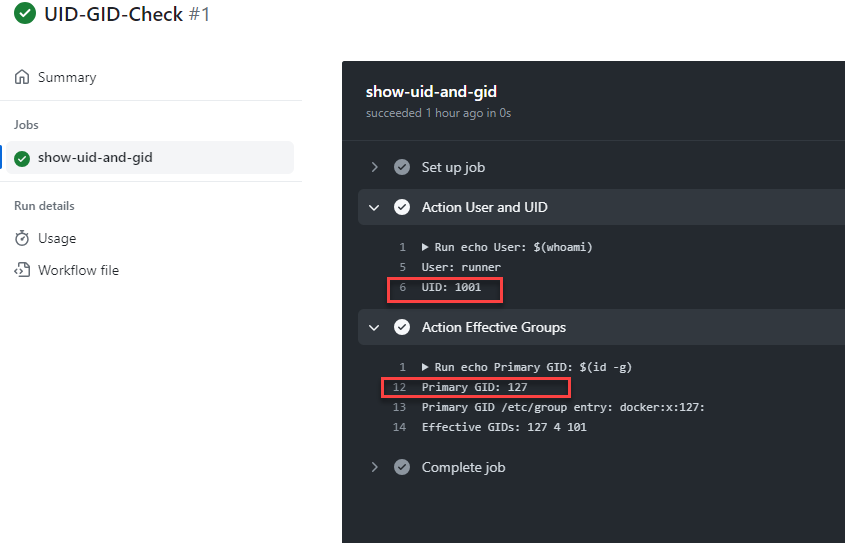
\includegraphics[width=\textwidth]{graphics/uidgid.png}
    \label{fig:uidgid}
\end{figure}
